
\subsection{Asymptotic expansion}

The first $2M$ terms of Hankel's expansion for $z \to \infty$ are given by
\begin{equation}
    J_\nu(z)
    \sim \sqrt{\frac{2}{\pi z}} \left( 
        \cos\left(\mu\right) \sum_{\ell=0}^{M-1} (-1)^\ell \frac{a_{2\ell}(\nu)}{z^{2\ell}}
        - \sin\left(\mu\right) \sum_{\ell=0}^{M-1} (-1)^\ell \frac{a_{2\ell+1}(\nu)}{z^{2\ell+1}}
        \right)
\end{equation}
where $\mu := z - \frac{(2\nu+1)\pi}{4}$ and 
\begin{equation}
    a_\ell(\nu) := \frac{(4\nu^2 - 1)(4\nu^2 - 3)\dots(4\nu^2 - (2\ell-1)^2)}{\ell! 8^\ell}.
\end{equation}

\red{Matvec evaluation with the NUFFT}

\red{Error bound}

\subsection{Local expansion}

If one looks at a rectangle $[0, \Omega] \times [0, R]$ where $\Omega R$ is
sufficiently small, $J_\nu(\omega r)$ is approximately low-rank for all $\omega
\in [0, \Omega], r \in [0, R]$. Fortuitously, one such low-rank approximation is
available in closed form \cite{wimp1962polynomial}
\begin{align}
    J_\nu(\omega r) = \sum_{\ell=0}^\infty \delta_\ell C_{2\ell}(\omega R) T_{2\ell}\left( \frac{r}{R} \right)
\end{align}

\begin{lemma} \label{lem:wimp} Truncating the Wimp expansion after $L$ terms
    gives
    \begin{equation}
        \abs{J_\nu(\omega r) - \sum_{\ell=0}^L C_{2\ell}(\omega R) T_{2\ell}\left( \frac{r}{R} \right)} 
        \leq \frac{2\exp\left\{ \frac{\nu}{2}(\beta - \gamma) + (L+1)(\beta + \gamma) \right\}}{1 - e^{\beta + \gamma}}
    \end{equation}
    for all $\omega \in [0, \Omega], r \in [0, R]$, where
    \begin{align}
        \psi(p) &:= \log p + \sqrt{1 - p^2} - \log\left( 1 + \sqrt{1 - p^2} \right) \\
        \beta &:= \psi\left( \frac{\Omega R}{\nu + 2L + 2} \right) \\
        \gamma &:= \begin{cases}
            \psi\left( \frac{\Omega R}{2L + 2 - \nu} \right) & L + 1 \geq \frac{\nu}{2} \\
            0 & \text{otherwise}
        \end{cases}
    \end{align}
\end{lemma}
\begin{proof}
    For $\nu$ even, the truncation error after $L$ terms is bounded by
    \begin{align}
        \abs{\sum_{\ell=L+1}^\infty C_{2\ell}(\omega R) T_{2\ell}\left( \frac{r}{R} \right)}
        &\leq 2\sum_{\ell=L+1}^\infty \abs{J_{\frac{\nu}{2} + \ell}\left(\frac{\omega R}{2}\right)} \abs{J_{\frac{\nu}{2} - \ell}\left(\frac{\omega R}{2}\right)}.
    \end{align}
    Define $p_\ell(\omega) := \omega R / (\nu + 2\ell)$. Then by Siegel's bound
    \cite[10.14.5]{olver2010nist} we have
    \begin{align}
        \abs{J_{\frac{\nu}{2} + \ell}\left(\frac{\omega R}{2}\right)}
        &= \abs{J_{\frac{\nu}{2} + \ell}\bigg(\Big(\frac{\nu}{2} + \ell\Big) p_\ell(\omega)\bigg)} \\
        &\leq \exp\left\{ \Big(\frac{\nu}{2} + \ell\Big) \psi\big(p_\ell(\omega)\big)\right\} \\
        &\leq \exp\left\{ \Big(\frac{\nu}{2} + \ell\Big) \beta \right\},
    \end{align}
    where the last inequality follows from the fact that $\psi$ is an increasing
    function on $(0,1)$, and thus $\psi\big(p_\ell(\omega)\big) \leq \beta < 0$
    for all $\ell \geq L+1$ and all $\omega \in [0, \Omega]$. 
    
    If $L+1 \geq \frac{\nu}{2}$, we define $q_\ell(\omega) := \omega R / (2\ell
    - \nu)$ and apply Siegel's bound again to obtain
    \begin{align}
        \abs{J_{\frac{\nu}{2} - \ell}\left(\frac{\omega R}{2}\right)}
        &= \abs{J_{\ell - \frac{\nu}{2}}\bigg(\Big(\ell - \frac{\nu}{2}\Big) q_\ell(\omega)\bigg)} 
        \leq \exp\left\{ \Big(\ell - \frac{\nu}{2}\Big) \gamma \right\}.
    \end{align}
    If $L+1 < \frac{\nu}{2}$, Siegel's bound does not apply and we use instead
    the simple bound $\abs{J_{\frac{\nu}{2} - \ell}\left(\frac{\omega
    R}{2}\right)} \leq 1$, which is equivalent to taking $\gamma = 0$. 

    All that remains is to apply a geometric series argument
    \begin{align}
        \abs{J_\nu(\omega r) - \sum_{\ell=0}^L C_{2\ell}(\omega R) T_{2\ell}\left( \frac{r}{R} \right)}
        &\leq 2\sum_{\ell=L+1}^\infty \exp\left\{ \Big(\frac{\nu}{2} + \ell\Big) \beta + \Big(\ell - \frac{\nu}{2}\Big) \gamma \right\} \\
        &= 2\exp\left\{\frac{\nu}{2}(\beta - \gamma)\right\} \sum_{\ell=L+1}^\infty \left( e^{\beta + \gamma} \right)^\ell \\
        &= \frac{2\exp\left\{ \frac{\nu}{2}(\beta - \gamma) + (L+1)(\beta + \gamma) \right\}}{1 - e^{\beta + \gamma}}
    \end{align}
    A similar calculation can be carried out for $\nu$ odd.
\end{proof}

This result is rather opaque regarding the impact of the various parameters
because we have not utilized any bounds to simplify the function $\psi$.
However, it remains relatively tight for $\nu = 0$ and is sufficient for our
purposes, because given $z, L > 0$, Lemma \ref{lem:wimp} gives a bound on the
pointwise error in approximating any block of the matrix $J_\nu(\omega_j r_k)$
for which $\omega r \leq z$ using the $L$-term Wimp expansion.

\subsection{Determining the cutoff between expansions}

With these error bounds in hand, we precompute the following tables for
tolerances $\epsilon = \texttt{1e-4}, \dots, \texttt{1e-15}$, orders $\nu = 1,
\dots, 100$, and number of asymptotic expansion terms $M = 1, \dots, 20$
\begin{itemize}
    \item $z_{\nu, \epsilon}^M$ such that the $M$-term asymptotic expansion of
    $J_\nu(\omega r)$ is $\epsilon$-accurate for all $\omega r > z_{\nu,
    \epsilon}^M$
    \item $L_{\nu, \epsilon}^M$ such that the $L_{\nu, \epsilon}^M$-term Wimp
    expansion of $J_\nu(\omega r)$ is $\epsilon$-accurate for all $\omega r \leq
    z_{\nu, \epsilon}^M$
\end{itemize}
Therefore, for any order $\nu$ we can look up a pair of complementary local and
asymptotic expansions with error everywhere bounded by the requested tolerance
$\epsilon$. The only remaining free parameter is the number of asymptotic terms
$M$. This parameter is selected heuristically in our implementation as 
\begin{equation}
    M = \min\left(\flr{1 + \frac{\nu}{5} - \frac{\log_{10}(\epsilon)}{4}}, 20\right)
\end{equation}
according to numerical experiments which maximize speed by balancing the cost of
the local, asymptotic, and direct evaluations.

\subsection{Subdividing the matrix into blocks by expansion}

Having established error bounds which allow us to automatically select the
number of asymptotic terms $M$, local terms $L$, and crossover point $z$ given a
tolerance $\epsilon$ and order $\nu$, we now discuss how to subdivide the matrix
$\bm{A}$ into three sets of blocks, each of which can be efficiently evaluated
as described above
\begin{itemize}
    \item Asymptotic blocks $\mathscr{A} = \big\{ (J, K) : \omega_j r_k > z \
    \forall \ j \in J, \ k \in K \big\}$
    \item Local blocks $\mathscr{L} = \big\{ (J, K) : \omega_j r_k \leq z \
    \forall \ j \in J, \ k \in K \big\}$
    \item Direct blocks $\mathscr{D}$ which are small enough that no fast
    expansion is needed
\end{itemize}
The idea is to consider index pairs $(j,k)$ such that $\omega_j r_k \approx z$,
which divides the matrix so that the upper left block can be applied using the
local expansion, the lower right block using the asymptotic expansion, and the
remaining two blocks can be evaluated directly or hierarchically subdivided.
This method converges for any such choice of $(j,k)$, but for efficiency they
are chosen to maximize the number of matrix entries which can be applied using a
fast expansion.

We start by initializing $\mathscr{A} = \mathscr{L} = \{\}$ and $\mathscr{D} =
\{(1:m, 1:n)\}$. The algorithm then proceeds iteratively as follows for each box
$(j_0:j_1, k_0:k_1) \in \mathscr{D}$
\begin{itemize}
    \item Compute $(j,k)$ which solves
    \begin{align}
        \text{maximize} &\quad (j-j_0)(k_1-k) + (j_1-j)(k-k_0) \\
        \text{such that} &\quad j_0 \leq j \leq j_1 \nonumber \\ 
        &\quad k_0 \leq k \leq k_1 \nonumber \\ 
        &\quad \omega_j r_k \leq z \nonumber
    \end{align}
    \item Remove $(j_0:j_1, k_0:k_1)$ from $\mathscr{D}$
    \item Add $(j+1:j_1, k+1:k_1)$ to $\mathscr{A}$ 
    \item Add $(j_0:j, k_0:k)$ to $\mathscr{L}$ 
    \item Add $(j_0:j, k+1:k_1)$ and $(j+1:j_1, k_0:k)$ to $\mathscr{D}$ 
\end{itemize}
We repeat the above subdivision scheme until all remaining boxes in
$\mathscr{D}$ are small enough to be evaluated directly.

\begin{figure}
    \centering
    \includegraphics[width=0.23\textwidth]{./figures/nufht_boxes_lvl1.pdf}
    \hfill
    \includegraphics[width=0.23\textwidth]{./figures/nufht_boxes_lvl2.pdf}
    \hfill
    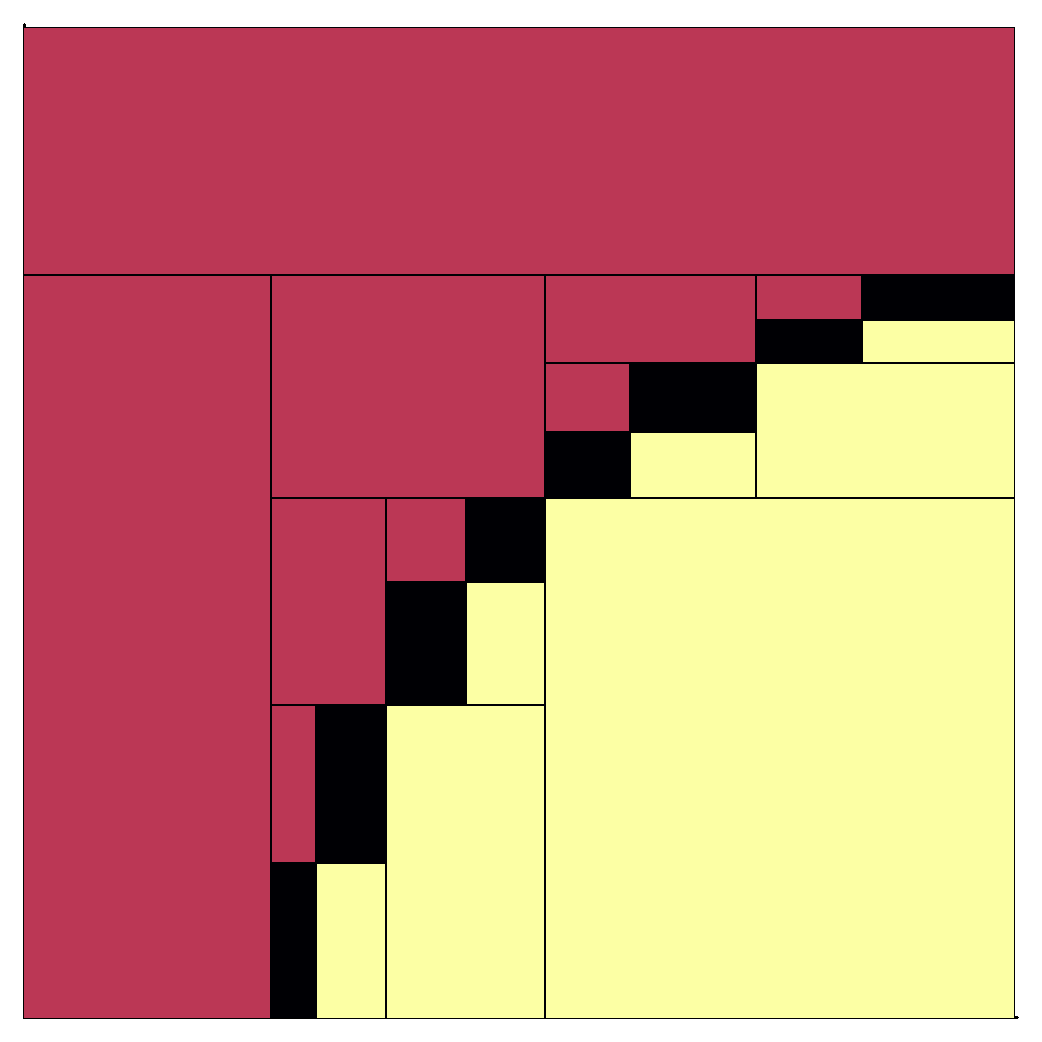
\includegraphics[width=0.23\textwidth]{./figures/nufht_boxes_lvl3.pdf}
    \hfill
    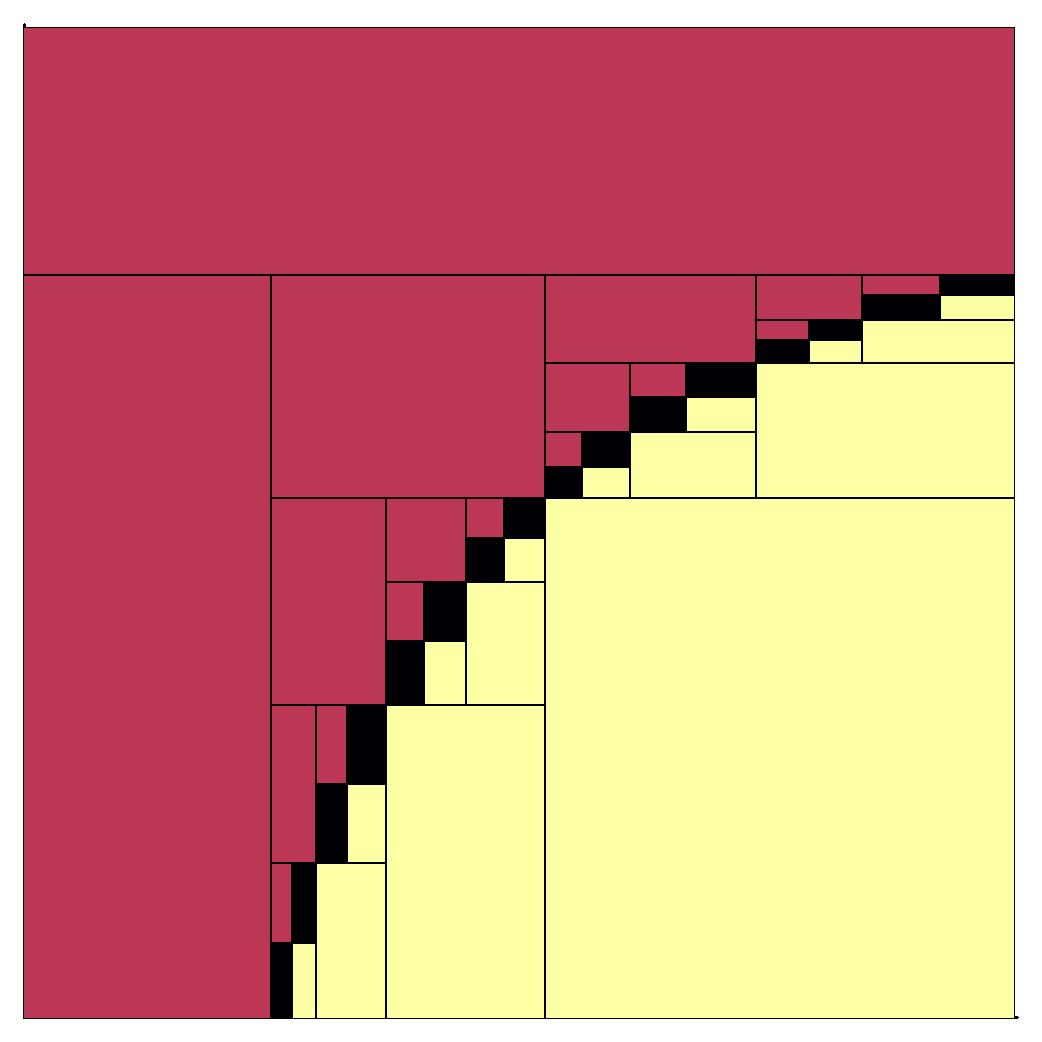
\includegraphics[width=0.23\textwidth]{./figures/nufht_boxes_lvl4.pdf}
    \caption{Direct (black), local (red), and asymptotic (yellow) boxes of
    $J_\nu(\omega_j r_k)$}
\end{figure}

\subsection{Computational complexity}

If $\omega_j r_k \leq z$ for all $j=1,\dots,n$ and $k=1,\dots,m$ then only the
low-rank local expansion is used, resulting in $\bO(m + n)$ complexity. If
instead $\omega_j r_k > z$ everywhere, then only the asymptotic expansion is
used, giving $\bO(m + n\log n)$ complexity. The third case, in which $\bm{A}$ is
subdivided in a non-trivial way, is more nuanced. \red{Complexity analysis for
subdivided case}